\subsection{Selected free live-tool examples}\label{app:gh-live}
The user saved four examples during free testing with visible predictions and model selection. All have accepted detection. Stored points are replayed through the 835-input reference and G/H rotation model. Saved model hashes, predictions and input vectors are checked; no redetection or fitting occurs.

\begin{table}[h]\centering\small
\caption{Identical stored landmarks through both models. Intended letters are user annotations. View labels were assigned visually, not by an independent ASL expert.}
\begin{tabular}{cllll}\toprule
Example & Intended & Visible view & Reference & G/H rotation\\\midrule
\tableinput gh_live_diagnostics_rows_nl.tex
\bottomrule\end{tabular}\end{table}
\begin{figure}[h]\centering
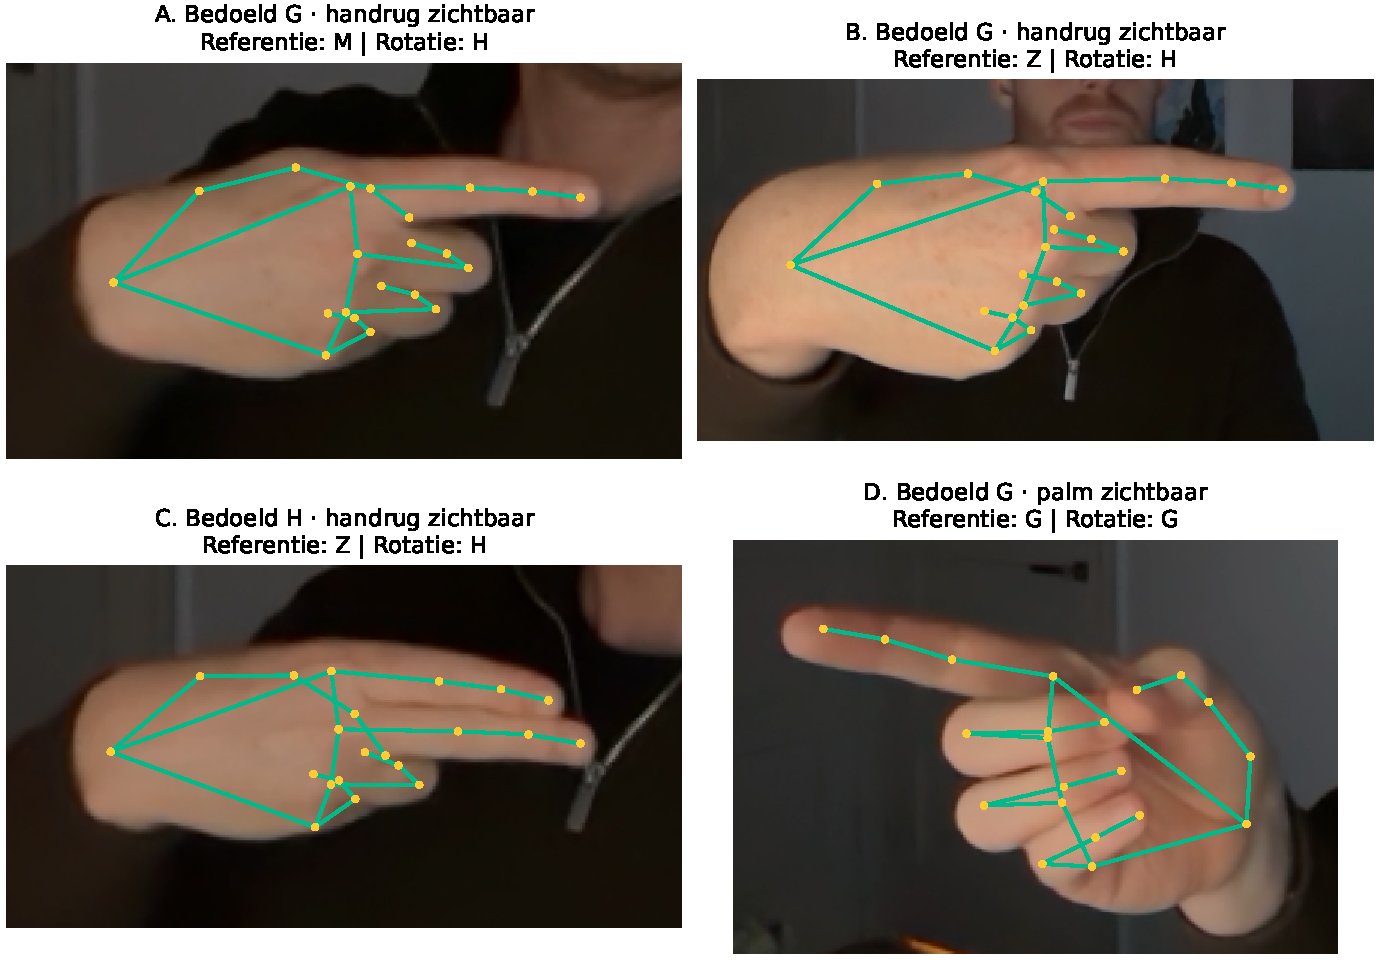
\includegraphics[width=.83\linewidth]{figures/gh_live_diagnostics.pdf}
\caption{All four new captures, cropped with their original landmarks. A/B: intended G remains H; C: H recovered; D: G recognized with palm visible. Reference/Rotation are model outputs, not confidence estimates.}
\label{fig:gh-live-diagnostics}
\end{figure}

\paragraph{Difference from the artificial test.}
Rigid rotation preserves intrinsic joint geometry. A/B instead have estimated middle DIP angles 161.7 and 164.7 degrees, compared with median 113.2 in 2,430 G fitting sources (middle 50\%: 109.2--118.2). Signed thumb deviations are $-1.9$ and $2.7$ degrees versus median 35.9. D measures 120.0 and 29.7 degrees respectively. These are world-point estimates, not true 3D anatomy. Pose, viewpoint and detector error cannot be separated here, nor does the comparison establish one angle as the cause of misclassification.

The high artificial score does not directly transfer: H is recovered but both hand-back Gs remain H. Rotation is not a demonstrated solution to the observed live confusion. Four selected images do not estimate representative precision, F1 or error frequency. Sources, measurements and hashes: \path{results/gh_live_diagnostics_20261107/}.
